\documentclass[hyperref={pdfpagelabels=false}]{beamer}	

\usepackage[brazil, portuges]{babel} % pacote português brasileiro
\usepackage[utf8]{inputenc} % pacote para acentuação direta
\usepackage{lmodern}
%\usepackage{multimedia} % pacote para utilizar vídeos
\usepackage{epigraph} % para utilizar epígrafes
\usepackage{graphicx}
\usepackage[3D]{movie15}

\usetheme{CambridgeUS}

\title{Dalle Pad}
    \subtitle{O gadget que te transforma em um DJ}
    \titlegraphic{
\includegraphics[scale=0.2]{Imagens/Logo01.png}}
    
\author{Leonardo Winter Pereira \newline Lucas Zimmermann Cordeiro \newline Luís Felipe Mazzuchetti Ortiz}

\date{\today}

\begin{document}

    \begin{frame}
        \titlepage
    \end{frame}

    \begin{frame}\frametitle{Índice}
        \tableofcontents
    \end{frame}

    \section{Componentes e custos}

        \begin{frame}\frametitle{Dalle Pad}

            \begin{figure}
                    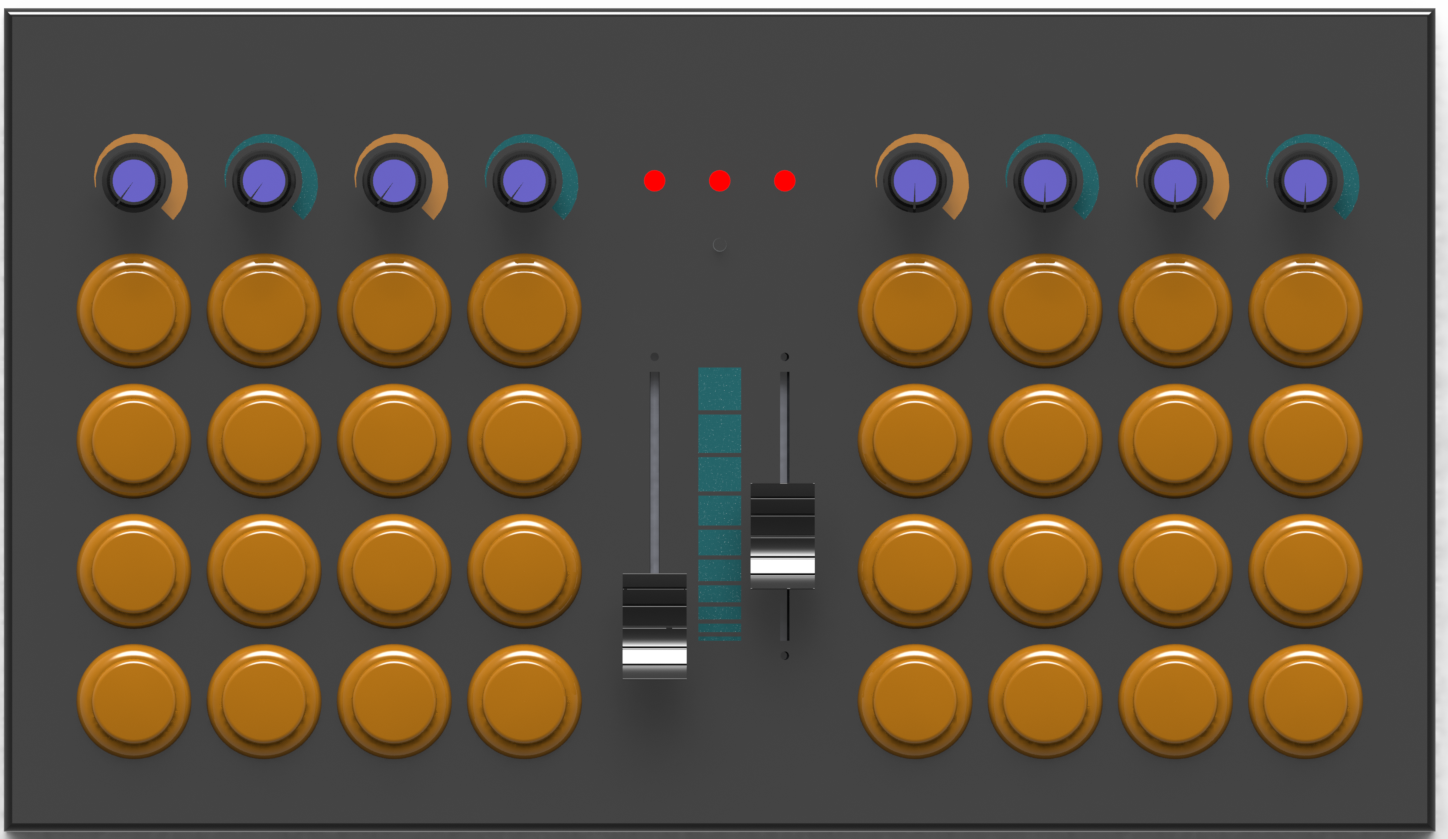
\includegraphics[scale=0.22]{Imagens/SW_Images/dalle_pad_montado2.png}
            \end{figure}

        \end{frame}

        \subsection{Potenciômetro linear B10K}

   	        \begin{frame}\frametitle{Potenciômetro linear B10K}

      	          \begin{itemize}
           	          \item Quantidade: 10 unidades;
            	      \item Custo do componente: US \$2,17 ; R\$ 8,13;
        	          \item Custo de entrega: US \$0,00 ; R\$ 0,00;
        	          \item Tamanho: 15mm;
         	      \end{itemize}

	              \begin{figure}
         	          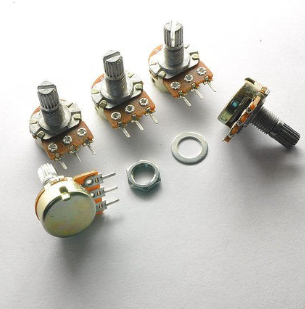
\includegraphics[scale=0.5]{Imagens/Apresentacao_2/potenciometro.png}
    	       	  \end{figure}	

   	     \end{frame}

        \subsection{Potenciômetro Mixer Fader B10K}

        	\begin{frame}\frametitle{Potenciômetro Mixer Fader B10K}

      	          \begin{itemize}
       	             \item Quantidade: 10 unidades;
        	         \item Custo do componente: US \$9,99 ; R\$ 37,46;
    	             \item Custo de entrega: US \$2,63 ; R\$ 9,86;
    	             \item Tamanho: 75mm x 9,5mm x 6,5mm;
         	      \end{itemize}

            	  \begin{figure}
                        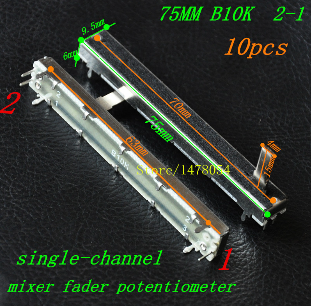
\includegraphics[scale=0.5]{Imagens/Apresentacao_2/mixerfader.png}
                  \end{figure}	

           	\end{frame}

        \subsection{Botão interruptor com parafuso}

            \begin{frame}\frametitle{Botão interruptor com parafuso}

      	          \begin{itemize}
       	             \item Quantidade: 48 unidades;
        	         \item Custo do componente: US \$8,40 ; R\$ 31,50;
    	             \item Custo de entrega: US \$19,04 ; R\$ 71,40;
    	             \item Tamanho: 24mm;
         	      \end{itemize}

        	      \begin{figure}
                        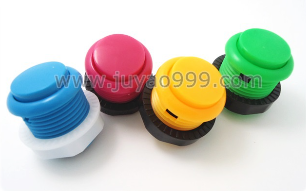
\includegraphics[scale=0.5]{Imagens/Apresentacao_2/botoes.png}
            	  \end{figure}	

           	\end{frame}

        \subsection{Invólucro}

            \begin{frame}\frametitle{Invólucro}

          	          \begin{itemize}
           	            \item Plástico;
            		          \begin{itemize}
            			         \item Fiel ao projeto mecânico;
                                 \item Custo Elevado.
            		          \end{itemize}
            	         \item Madeira;
                              \begin{itemize}
            			         \item Baixo custo;
                                 \item Necessidade de produzir a peça manualmente.
            		          \end{itemize}
        	             \item Acrílico;
                              \begin{itemize}
            			         \item Baixo custo;
                                 \item Quando comparado com a madeira, apresenta maior complexidade na perfuração.
            		          \end{itemize}
             	      \end{itemize}

           	     \end{frame}

    \section{Etapas do projeto}

        \begin{frame}\frametitle{Etapas do projeto}

      	     \begin{itemize}
       	        \item Quatro etapas:
                    \newline
    		      \begin{itemize}
    			     \item Primeira etapa - 15.04.2016;
                        \newline
    			     \item Segunda etapa - 13.05.2016;
                        \newline
    			     \item Terceira etapa - 03.06.2016;
                        \newline
    			     \item Quarta etapa - 17.06.2016;
    		      \end{itemize}
         	 \end{itemize}

       	\end{frame}

        \subsection{Primeira etapa}

            \begin{frame}\frametitle{Primeira Etapa}

                \begin{itemize}
           	        \item Plano do projeto;
            	    \item Diagramas esquemáticos;
        	        \item Versão inicial do hardware;
             	\end{itemize}

            \end{frame}

        \subsection{Segunda etapa}

            \begin{frame}\frametitle{Segunda Etapa}

        	   \begin{itemize}
           	        \item Início do desenvolvimento do software;
            	    \item Confecção da PCB;
        	        \item Projetar o invólucro;
               \end{itemize}

            \end{frame}

        \subsection{Terceira etapa}

            \begin{frame}\frametitle{Terceira Etapa}

        	   \begin{itemize}
       	             \item Conexão entre software e hardware;
       	             \item Software apresentando funções básicas;
        	         \item Finalização do desenvolvimento do hardware;
               \end{itemize}

            \end{frame}

        \subsection{Quarta etapa}

            \begin{frame}\frametitle{Quarta Etapa}

        	   \begin{itemize}
       	             \item Aprimoramento do software e suas funções;
        	         \item Tempo para correção de possíveis imprevistos;
               \end{itemize}

            \end{frame}

    \section{Riscos}

    	 \begin{frame}\frametitle{Riscos}
    	
            \begin{itemize}
       	        \item Problemas com prazos de entrega de componentes encomendados que interrompam o andamento do projeto;
        	    \item Falta de conhecimento técnico sobre MIDI;
    	        \item Custo elevado ao utilizar a Impressora 3D do NUFER;
            \end{itemize}

        \end{frame}

        \subsection{Prazo de entrega}

           \begin{frame}\frametitle{Riscos}

        	   \begin{itemize}
        	       \item Problemas com prazos de entrega de componentes encomendados que interrompam o andamento do projeto;
        	           \begin{itemize}
           	     	        \item Mitigação: Encomendas devem ser feitas antecipadamente e sempre considerando a necessidade de peças extras;
            	       		\item Mitigação: Pode ser necessário a realização de outra compra em estabelecimentos locais, aumentando os custos do projeto;
        	           \end{itemize}
               \end{itemize}

           \end{frame}

        \subsection{Conhecimento sobre MIDI}

           \begin{frame}\frametitle{Riscos}

        	   \begin{itemize}
        	       \item Falta de conhecimento técnico sobre MIDI;
        	           \begin{itemize}
           	     	        \item Mitigação: A equipe deve procurar ler sobre o assunto antes mesmo do início do projeto. O gerente, principalmente, deve apresentar conhecimento técnico sobre todo o assunto.
        	           \end{itemize}
                \end{itemize}

           \end{frame}

        \subsection{Custo Impressora 3D}

           \begin{frame}\frametitle{Riscos}

        	   \begin{itemize}
        	       \item Custo elevado ao utilizar a Impressora 3D do NUFER;
        	           \begin{itemize}
           	     	        \item Mitigação: Aumento do orçamento base, visto a necessidade de utilizar um serviço terceirizado ou
            	         	\item Mitigação: Necessidade de confeccionar o invólucro com madeira ou acrílico, utilizando serviços terceirizados ou utilizando o próprio laboratório de Design / Mecânica da UTFPR;
        	           \end{itemize}
               \end{itemize}

            \end{frame}

\end{document} 